\documentclass[11pt,aspectratio=169]{beamer}
\usepackage[spanish,es-nodecimaldot]{babel}
\usepackage{fontspec}
\setsansfont{Inter 18pt}[BoldFont={Inter 18pt SemiBold}]
\renewcommand{\familydefault}{\sfdefault}
\usepackage{graphicx}
\usepackage{tikz}
\graphicspath{{sesion1/presentation/images/}{images/}}

\definecolor{tinta}{HTML}{191A20}
\definecolor{slotA}{HTML}{D9E1F2}
\definecolor{slotPhone}{HTML}{DDE7F0}
\definecolor{menticard}{HTML}{F5F5F5}

\setbeamercolor{normal text}{fg=tinta,bg=white}
\setbeamertemplate{navigation symbols}{}
\setbeamertemplate{headline}{}
\setbeamertemplate{footline}{}
\hyphenpenalty=10000
\exhyphenpenalty=10000

% Coordinates use the 1398x786 reference canvas.
\newcommand{\px}[1]{\dimexpr\paperwidth*#1/1398\relax}
\newcommand{\py}[1]{\dimexpr\paperheight*#1/786\relax}
\newcommand{\mentinode}[6]{%
  \node[anchor=north west,inner sep=0pt,outer sep=0pt,text width=\px{#3},align=left]
    at ([xshift=\px{#1},yshift=-\py{#2}]current page.north west)
    {{\color{tinta}\fontsize{#4}{#5}\selectfont #6}};%
}
\newcommand{\mentihint}{\mentinode{55}{560}{260}{8}{11}{Mentimeter $\rightarrow$}}

\begin{document}

% 1
\begin{frame}[plain]
  \begin{tikzpicture}[remember picture,overlay]
    \mentinode{54}{247}{1040}{30}{36}{¿Qué es la inteligencia}
    \mentinode{54}{353}{620}{30}{36}{artificial?}
    \node[anchor=north west,inner sep=0] at ([xshift=\px{760},yshift=-\py{375}]current page.north west)
      {
\includegraphics[width=\px{580}]{Smartphone by the Jungle River.png}};
  \end{tikzpicture}
\end{frame}

% 2
\begin{frame}[plain]
  \begin{tikzpicture}[remember picture,overlay]
    \mentinode{54}{291}{1280}{14.5}{19}{¿Qué sabes sobre la IA?}
    \mentinode{55}{443}{700}{8}{11}{Google Forms}
    \mentinode{55}{495}{700}{8}{11}{Enlace: https://shorturl.at/A8z29}
    \node[anchor=north west,inner sep=0] at ([xshift=\px{1000},yshift=-\py{315}]current page.north west)
      {
\includegraphics[width=\px{260},height=\py{260}]{qr.png}};
  \end{tikzpicture}
\end{frame}

% 3: word cloud in Mentimeter; cue is on slide 2.

% 4
\begin{frame}[plain]
  \begin{tikzpicture}[remember picture,overlay]
    \mentinode{54}{297}{610}{19.5}{24}{Inteligencia artificial}
    \mentinode{55}{435}{590}{8}{14}{Es una tecnología que permite a las computadoras realizar tareas como reconocer imágenes, comprender preguntas, recomendar contenido o crear contenido}
    \node[anchor=north west,inner sep=0] at ([xshift=\px{710},yshift=-\py{190}]current page.north west)
      {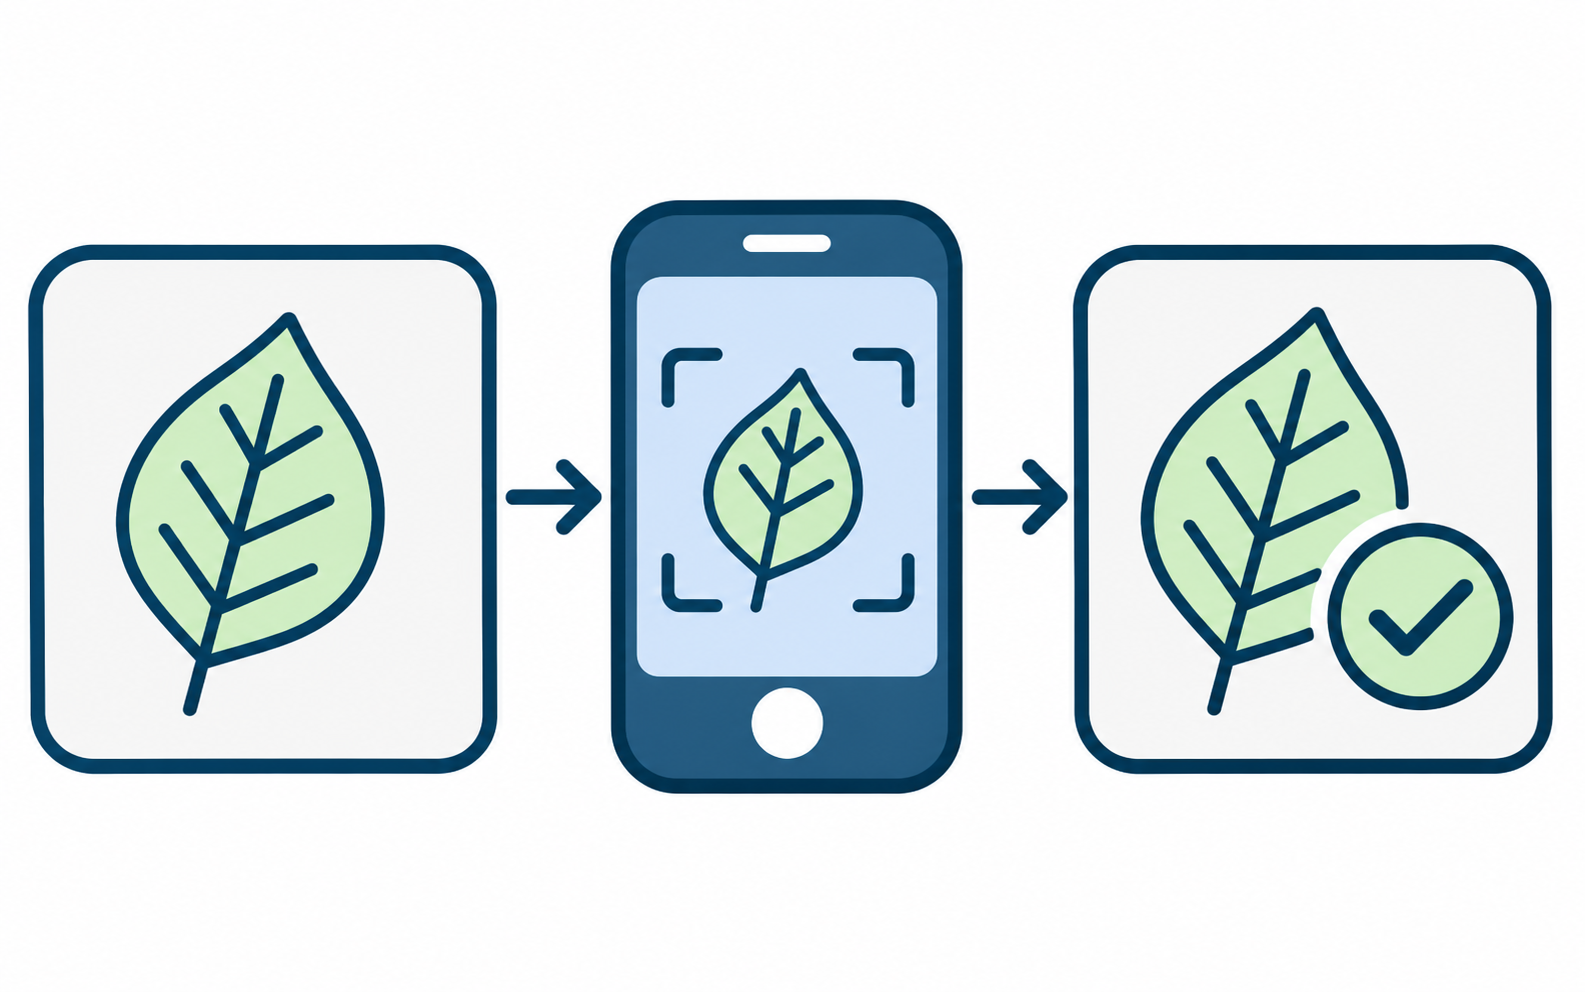
\includegraphics[width=\px{630}]{Leaf Scanning App Workflow.png}};
  \end{tikzpicture}
\end{frame}

% 5
\begin{frame}[plain]
  \begin{tikzpicture}[remember picture,overlay]
    \mentinode{54}{287}{590}{19.5}{24}{¿Dónde encontramos inteligencia artificial?}
    % \mentinode{55}{445}{590}{8}{14}{La IA puede estar presente en muchas actividades de nuestra vida}
    % \fill[slotA]
    %   ([xshift=\px{700}]current page.north west)
    %   rectangle (current page.south east);
    \begin{scope}
      \clip ([xshift=\px{700}]current page.north west) rectangle (current page.south east);
      \node[anchor=center,inner sep=0] at ([xshift=\px{1049},yshift=-\py{393}]current page.north west)
        {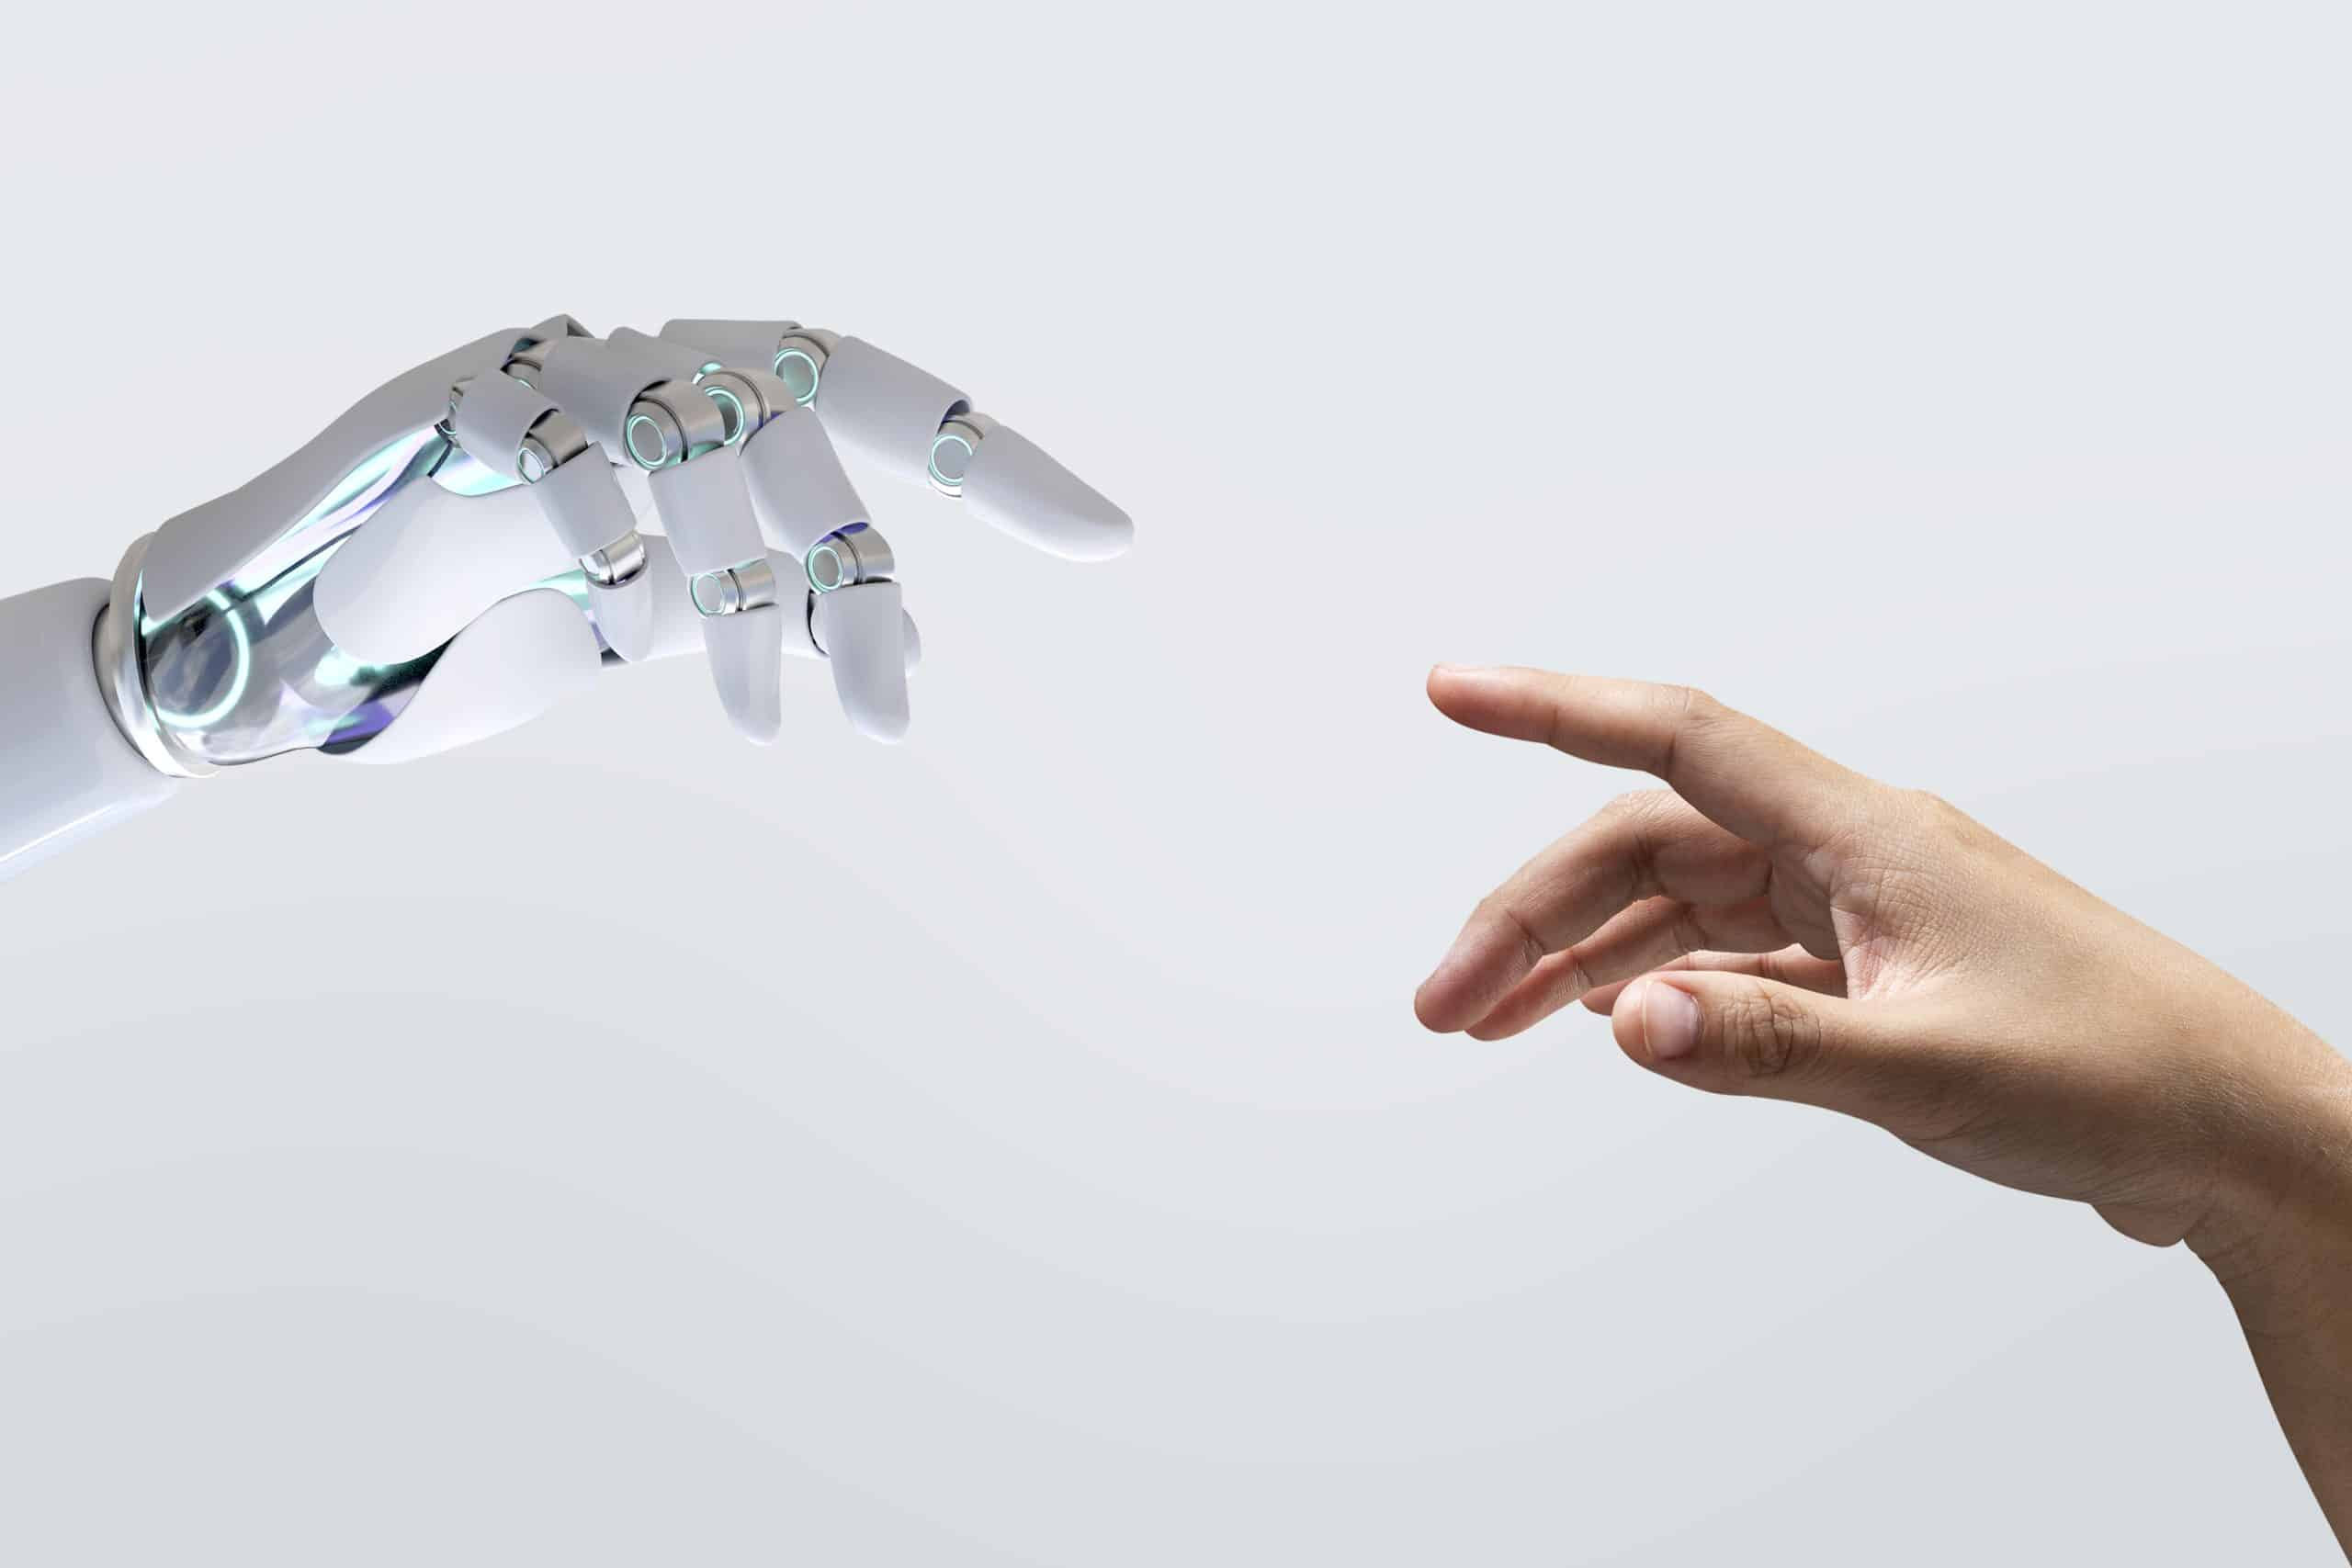
\includegraphics[height=\paperheight]{ai_touch.jpg}};
    \end{scope}
    \mentihint
  \end{tikzpicture}
\end{frame}

% 6--11: six image votes in Mentimeter; cue is on slide 5.

% 12
\begin{frame}[plain]
  \begin{tikzpicture}[remember picture,overlay]
    \mentinode{54}{331}{590}{19.5}{24}{La IA en nuestra vida cotidiana}
    % \fill[slotPhone]
    %   ([xshift=\px{710},yshift=-\py{78}]current page.north west)
    %   rectangle
    %   ([xshift=\px{1342},yshift=-\py{710}]current page.north west);
    \begin{scope}
      \clip ([xshift=\px{710},yshift=-\py{78}]current page.north west)
        rectangle ([xshift=\px{1342},yshift=-\py{710}]current page.north west);
      \node[anchor=center,inner sep=0] at ([xshift=\px{1026},yshift=-\py{394}]current page.north west)
        {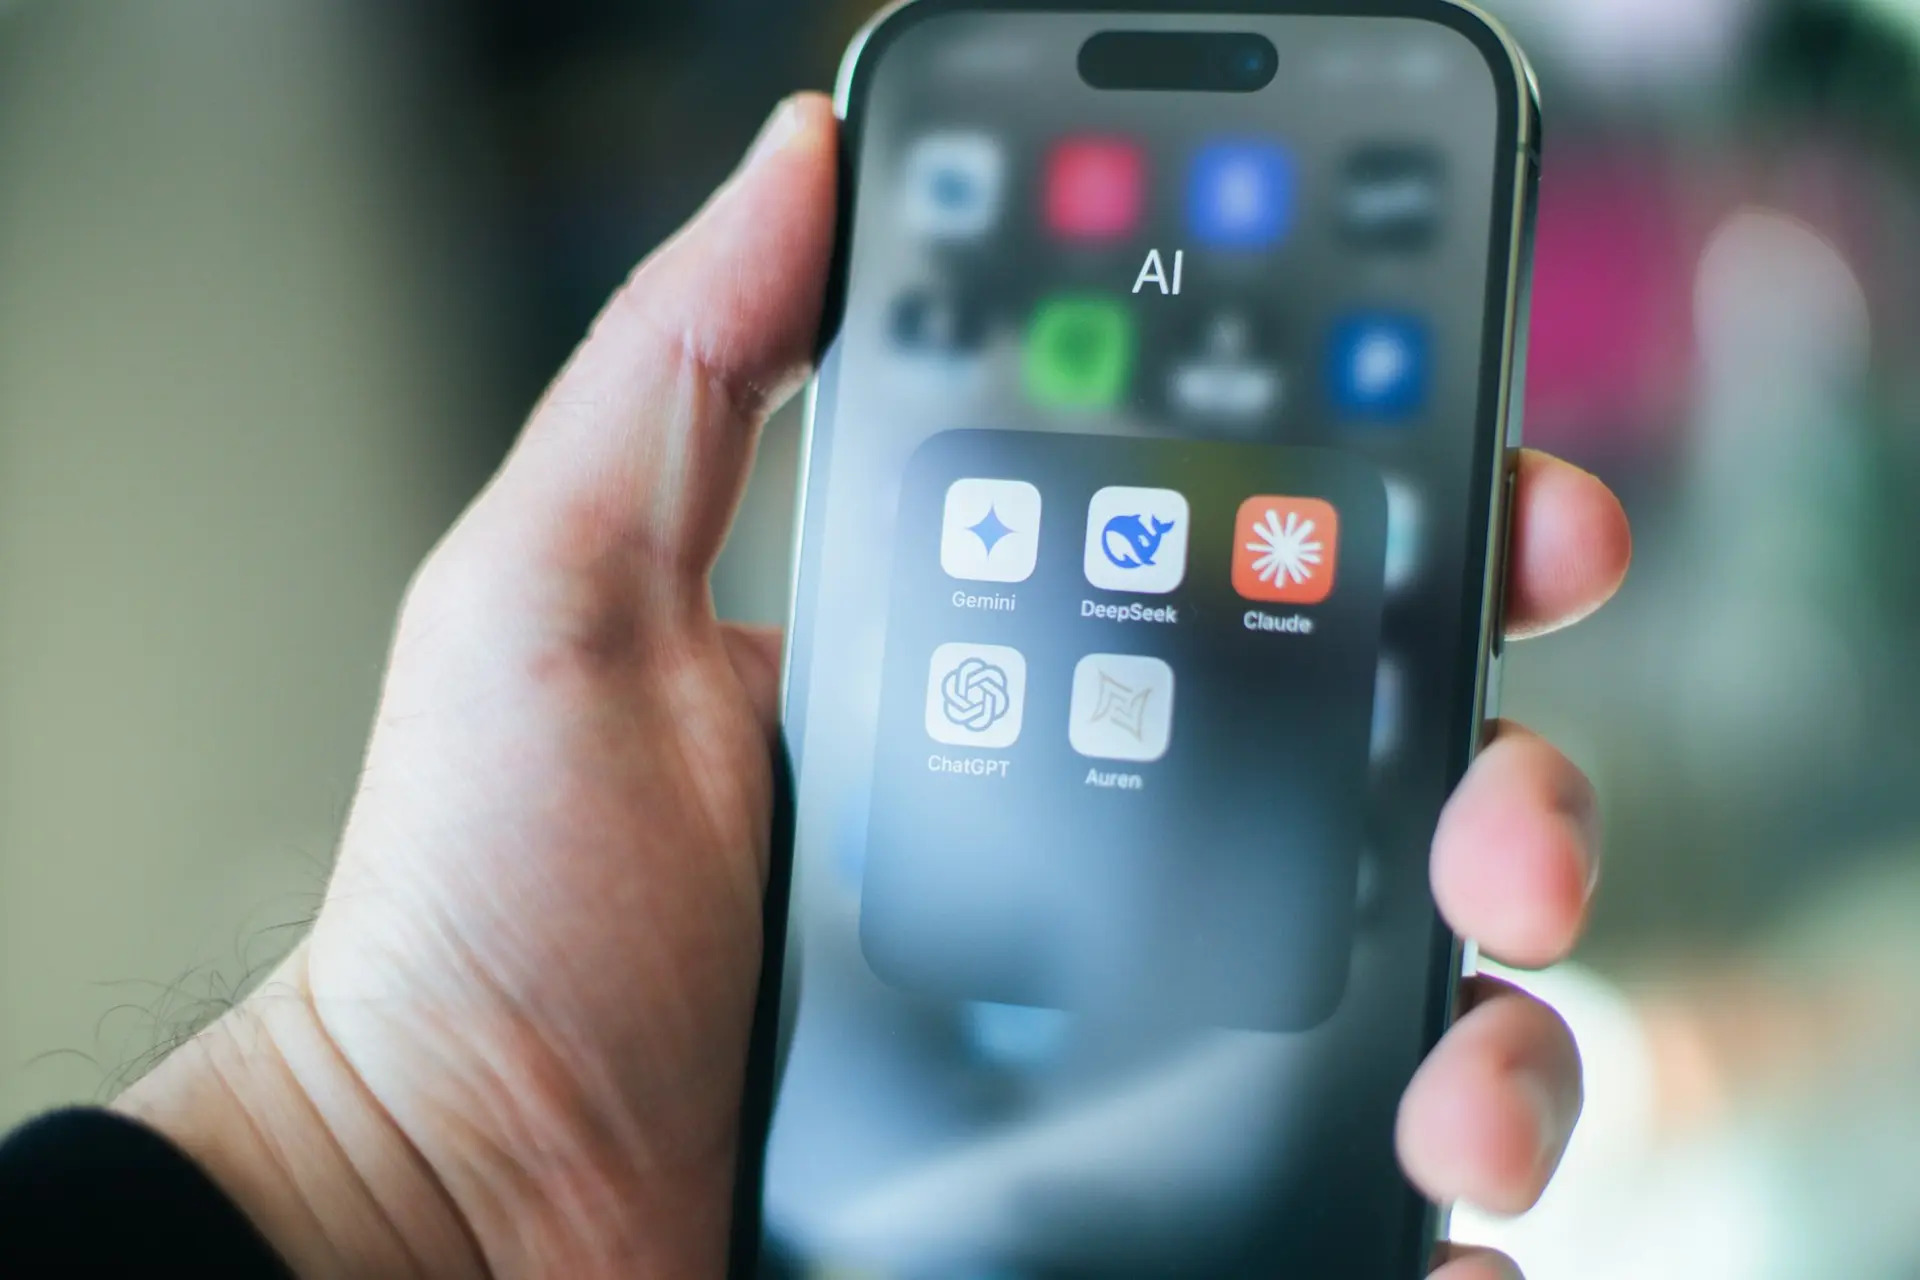
\includegraphics[height=\py{632}]{phone_ia.jpg}};
    \end{scope}
  \end{tikzpicture}
\end{frame}

% Después de la diapositiva 12: espacio para ejemplos reales.
\begin{frame}[plain]
  \begin{tikzpicture}[remember picture,overlay]
    \mentinode{54}{250}{1280}{19.5}{24}{Aplicaciones reales hechas con IA}
    \node[anchor=north west,inner sep=0] at ([xshift=\px{74},yshift=-\py{330}]current page.north west)
      {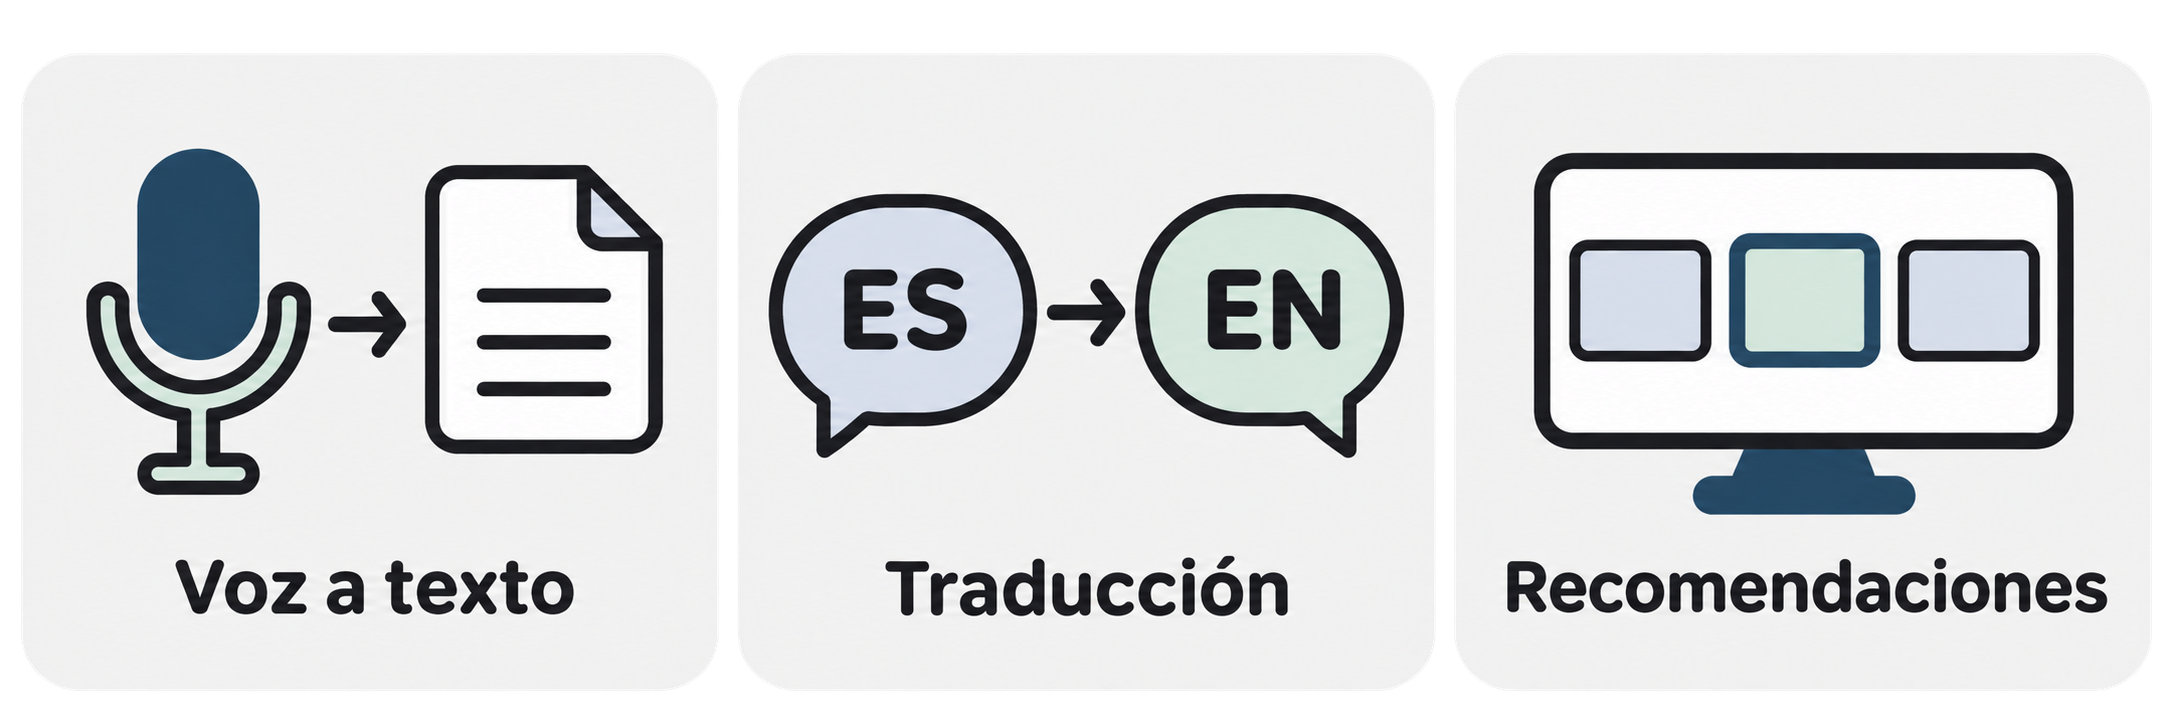
\includegraphics[width=\px{1250}]{Voz, traducción y recomendaciones.png}};
  \end{tikzpicture}
\end{frame}

% 13
\begin{frame}[plain]
  \begin{tikzpicture}[remember picture,overlay]
    \mentinode{54}{190}{1280}{20}{24}{No todo lo automático es IA}
    \mentinode{54}{405}{450}{10}{15}{La diferencia está en cómo decide: una regla fija o patrones aprendidos.}
    \node[anchor=north west,inner sep=0] at ([xshift=\px{580},yshift=-\py{275}]current page.north west)
      {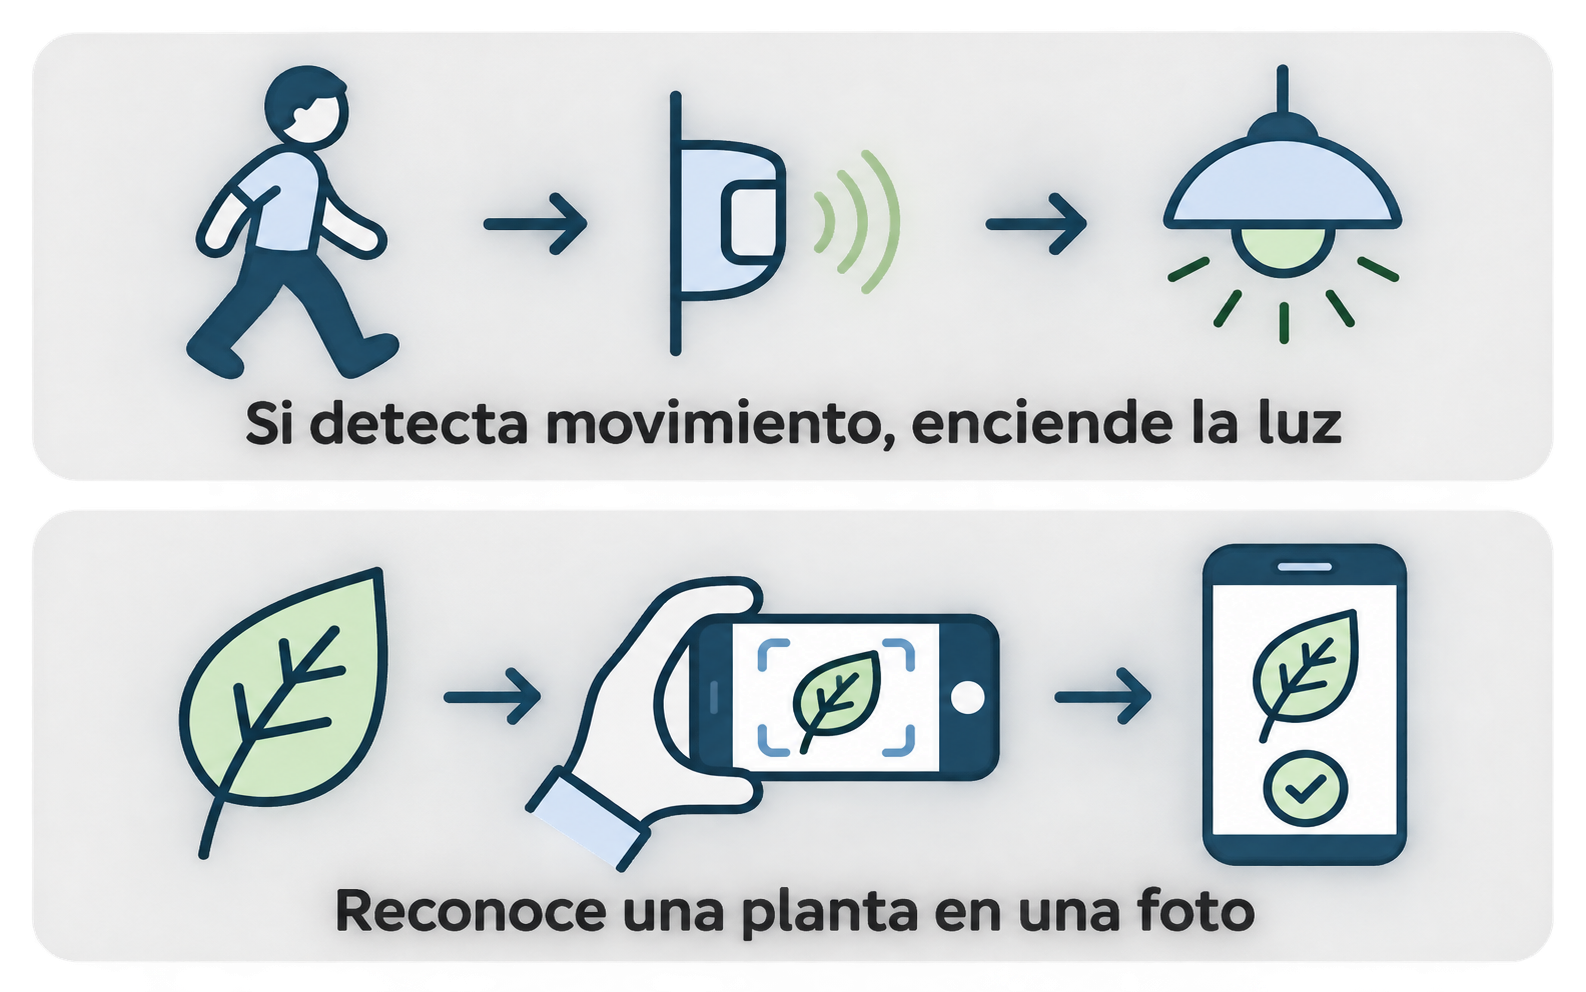
\includegraphics[width=\px{760}]{Automated Actions and Plant Recognition.png}};
  \end{tikzpicture}
\end{frame}

% 14
\begin{frame}[plain]
  \begin{tikzpicture}[remember picture,overlay]
    \mentinode{54}{297}{445}{19.5}{24}{IA en la Amazonía}
    \mentinode{55}{435}{440}{10}{15}{Puede ayudar a observar el entorno, organizar información y compartir ideas.}
    \node[anchor=north west,inner sep=0] at ([xshift=\px{550},yshift=-\py{175}]current page.north west)
      {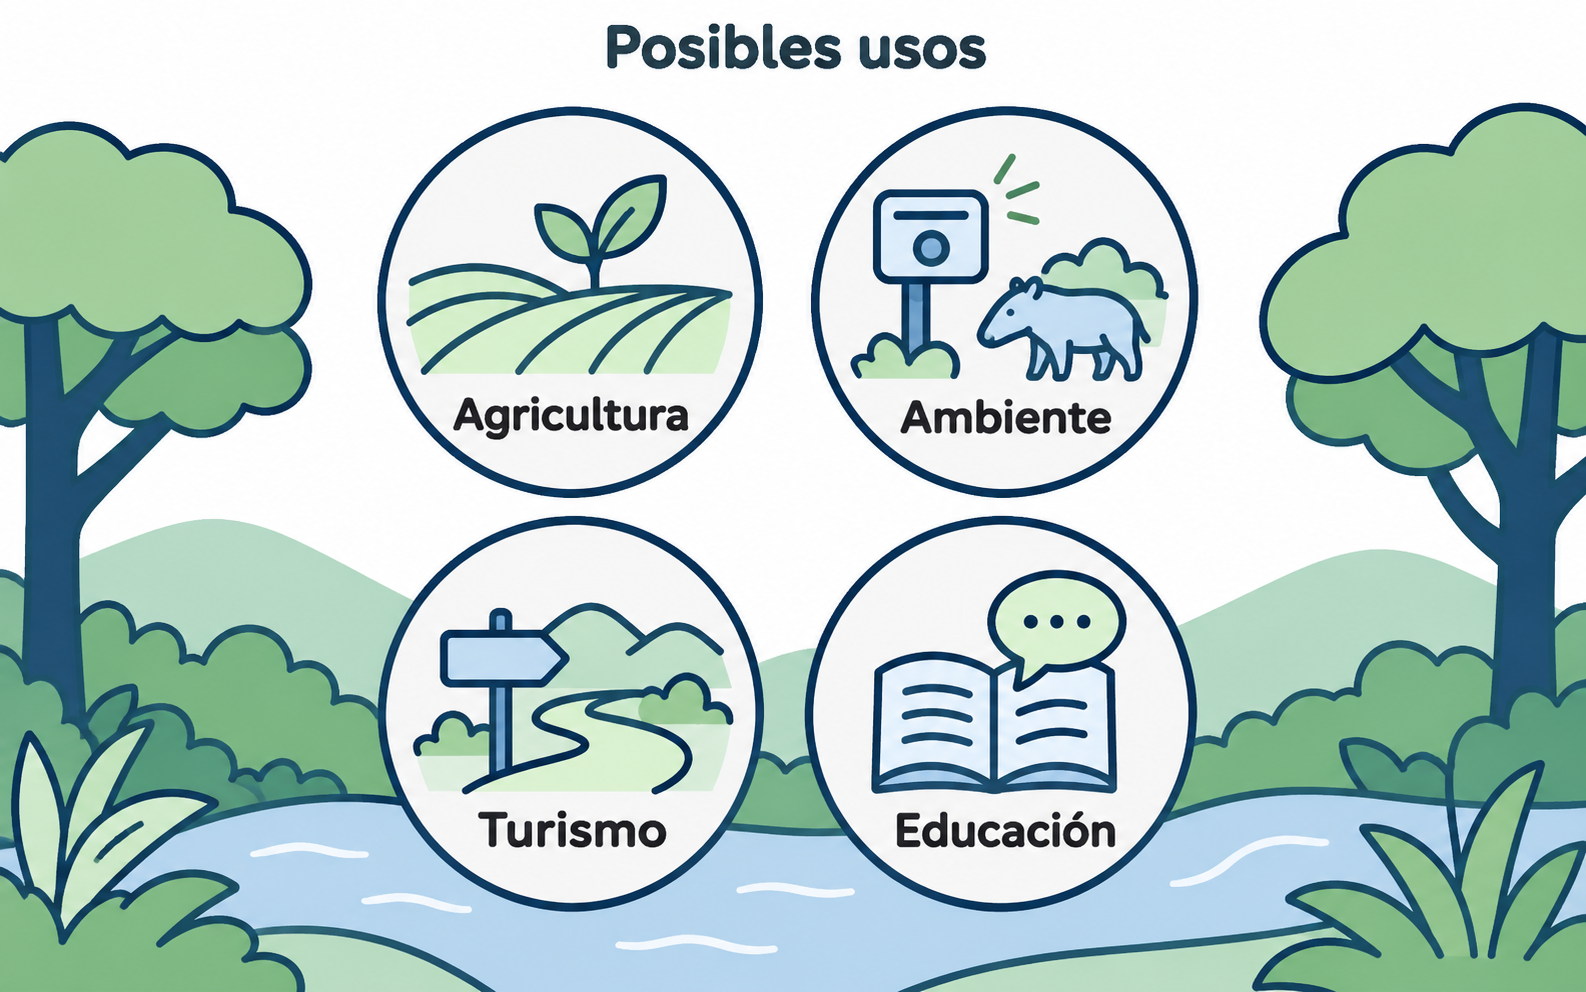
\includegraphics[width=\px{790}]{Posibles usos en la naturaleza.png}};
  \end{tikzpicture}
\end{frame}

% 15
\begin{frame}[plain]
  \begin{tikzpicture}[remember picture,overlay]
    \mentinode{54}{297}{445}{19.5}{24}{¿La IA siempre acierta?}
    \mentinode{55}{435}{440}{10}{15}{Antes de compartir una respuesta, comprueba fechas, cifras y nombres en una fuente confiable.}
    \node[anchor=north west,inner sep=0] at ([xshift=\px{550},yshift=-\py{175}]current page.north west)
      {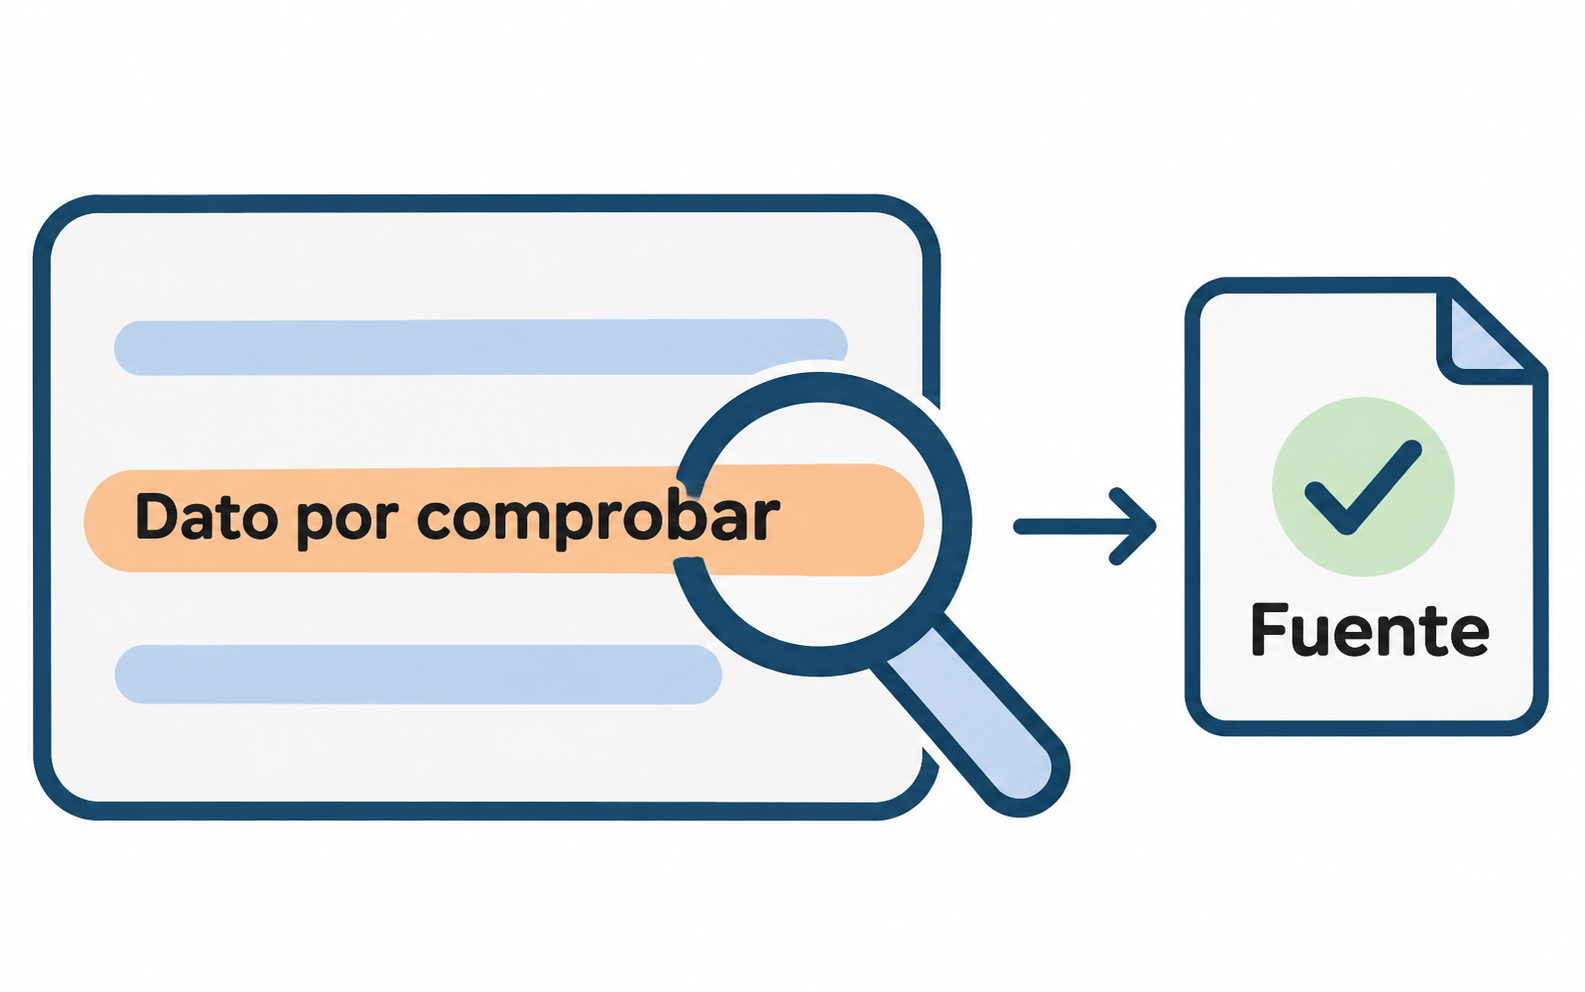
\includegraphics[width=\px{790}]{Verifying a Highlighted Data Point.png}};
  \end{tikzpicture}
\end{frame}

% 16
\begin{frame}[plain]
  \begin{tikzpicture}[remember picture,overlay]
    \mentinode{54}{297}{445}{19.5}{24}{Aprender con ejemplos}
    \mentinode{55}{435}{440}{10}{15}{Lo que aprende depende de la calidad y variedad de los ejemplos.}
    \mentinode{55}{610}{440}{8}{11}{Machine Learning \textbullet\ Deep Learning}
    \node[anchor=north west,inner sep=0] at ([xshift=\px{550},yshift=-\py{175}]current page.north west)
      {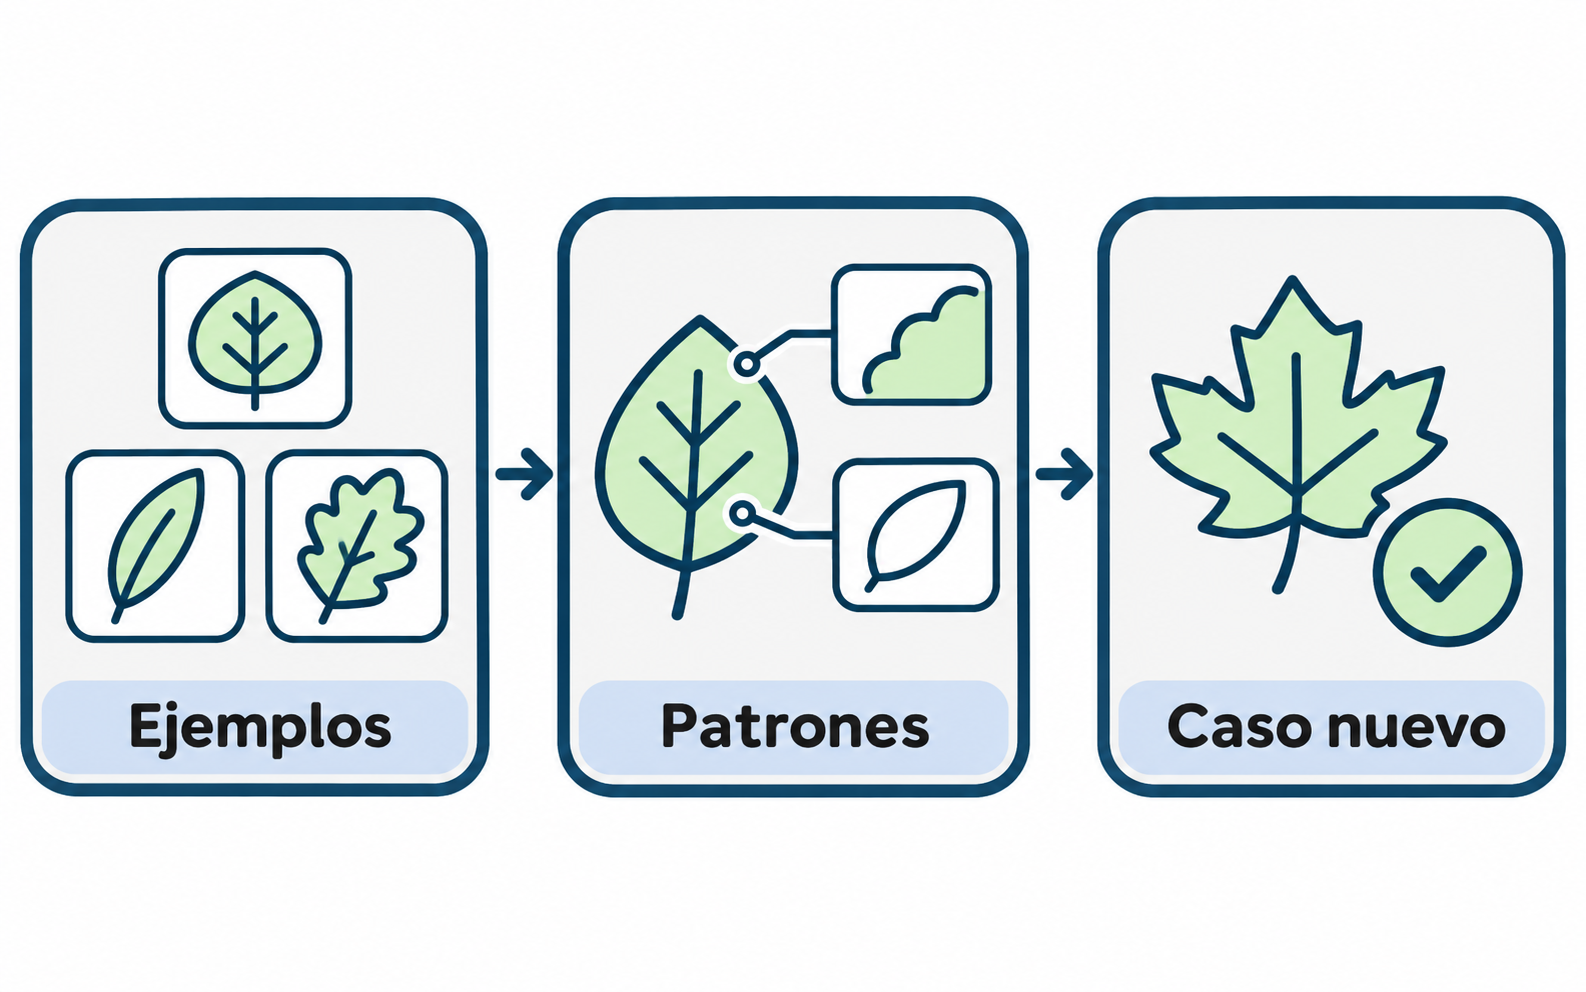
\includegraphics[width=\px{790}]{Leaf Pattern Identification Infographic.png}};
  \end{tikzpicture}
\end{frame}

% 17
\begin{frame}[plain]
  \begin{tikzpicture}[remember picture,overlay]
    \mentinode{54}{297}{445}{19.5}{24}{La IA también crea}
    \mentinode{55}{435}{440}{10}{15}{La instrucción orienta el resultado; siempre conviene revisarlo.}
    \node[anchor=north west,inner sep=0] at ([xshift=\px{550},yshift=-\py{175}]current page.north west)
      {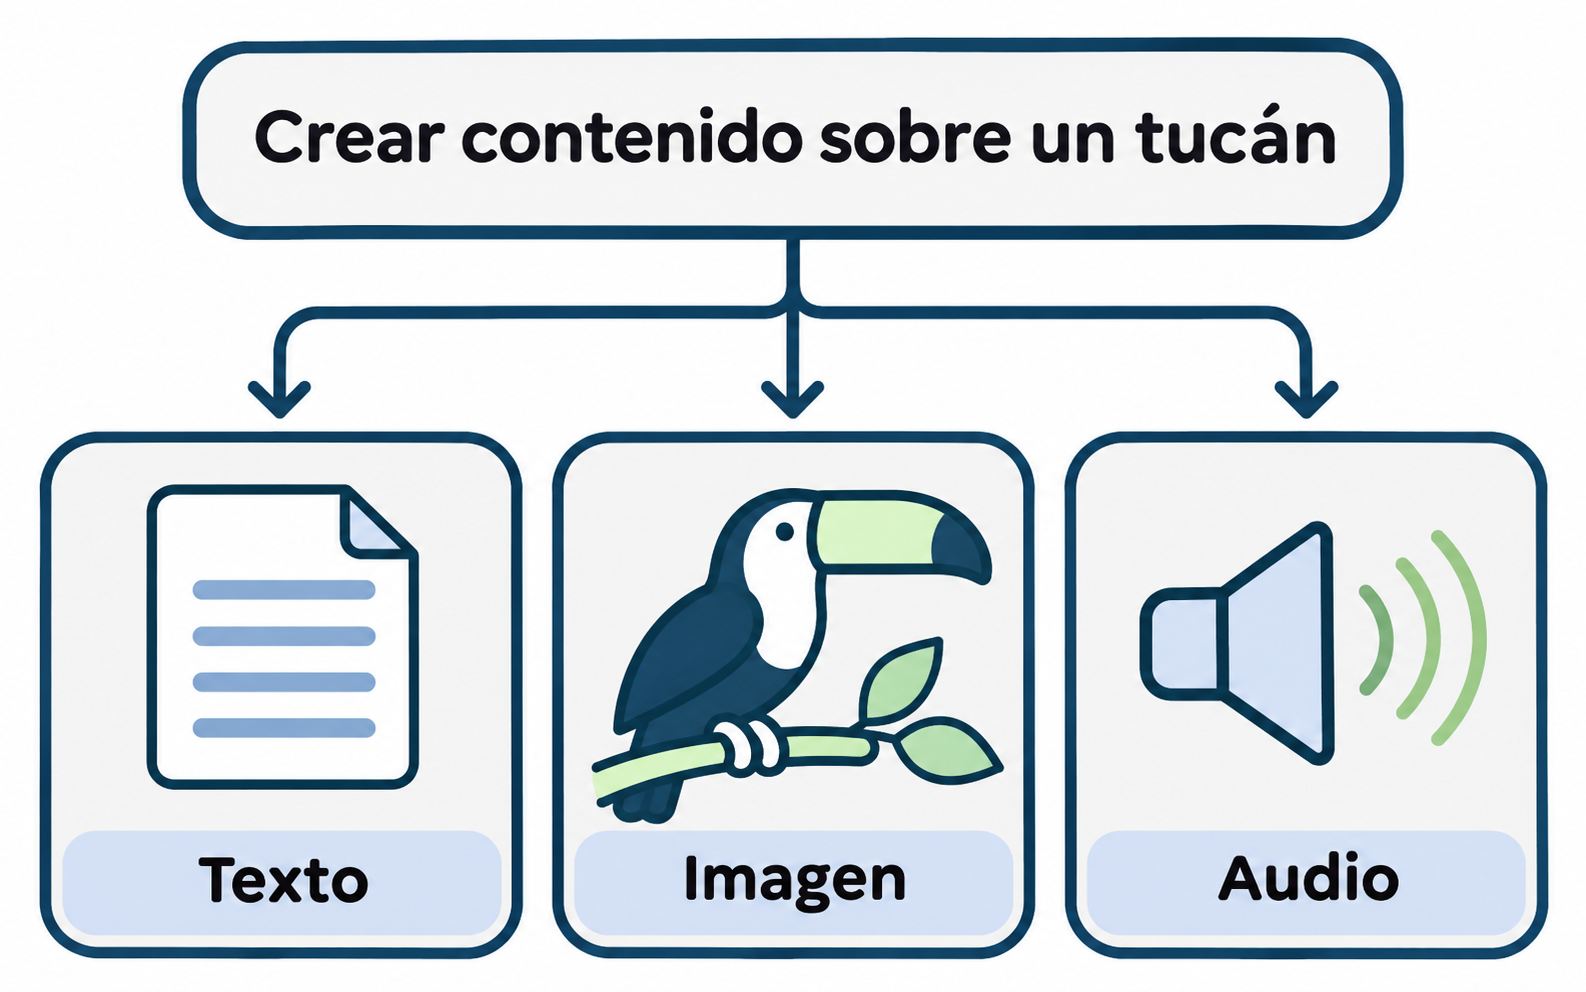
\includegraphics[width=\px{790}]{Tucán_ texto, imagen y audio.png}};
  \end{tikzpicture}
\end{frame}

% 18
\begin{frame}[plain]
  \begin{tikzpicture}[remember picture,overlay]
    \mentinode{54}{190}{1280}{20}{24}{¿Todas las IA pueden hacer lo mismo?}
    \mentinode{54}{405}{450}{10}{15}{Hacer bien una tarea no significa poder hacer todas.}
    \mentinode{54}{520}{450}{8}{11}{ANI: especializada \textbullet\ AGI: general}
    \node[anchor=north west,inner sep=0] at ([xshift=\px{580},yshift=-\py{275}]current page.north west)
      {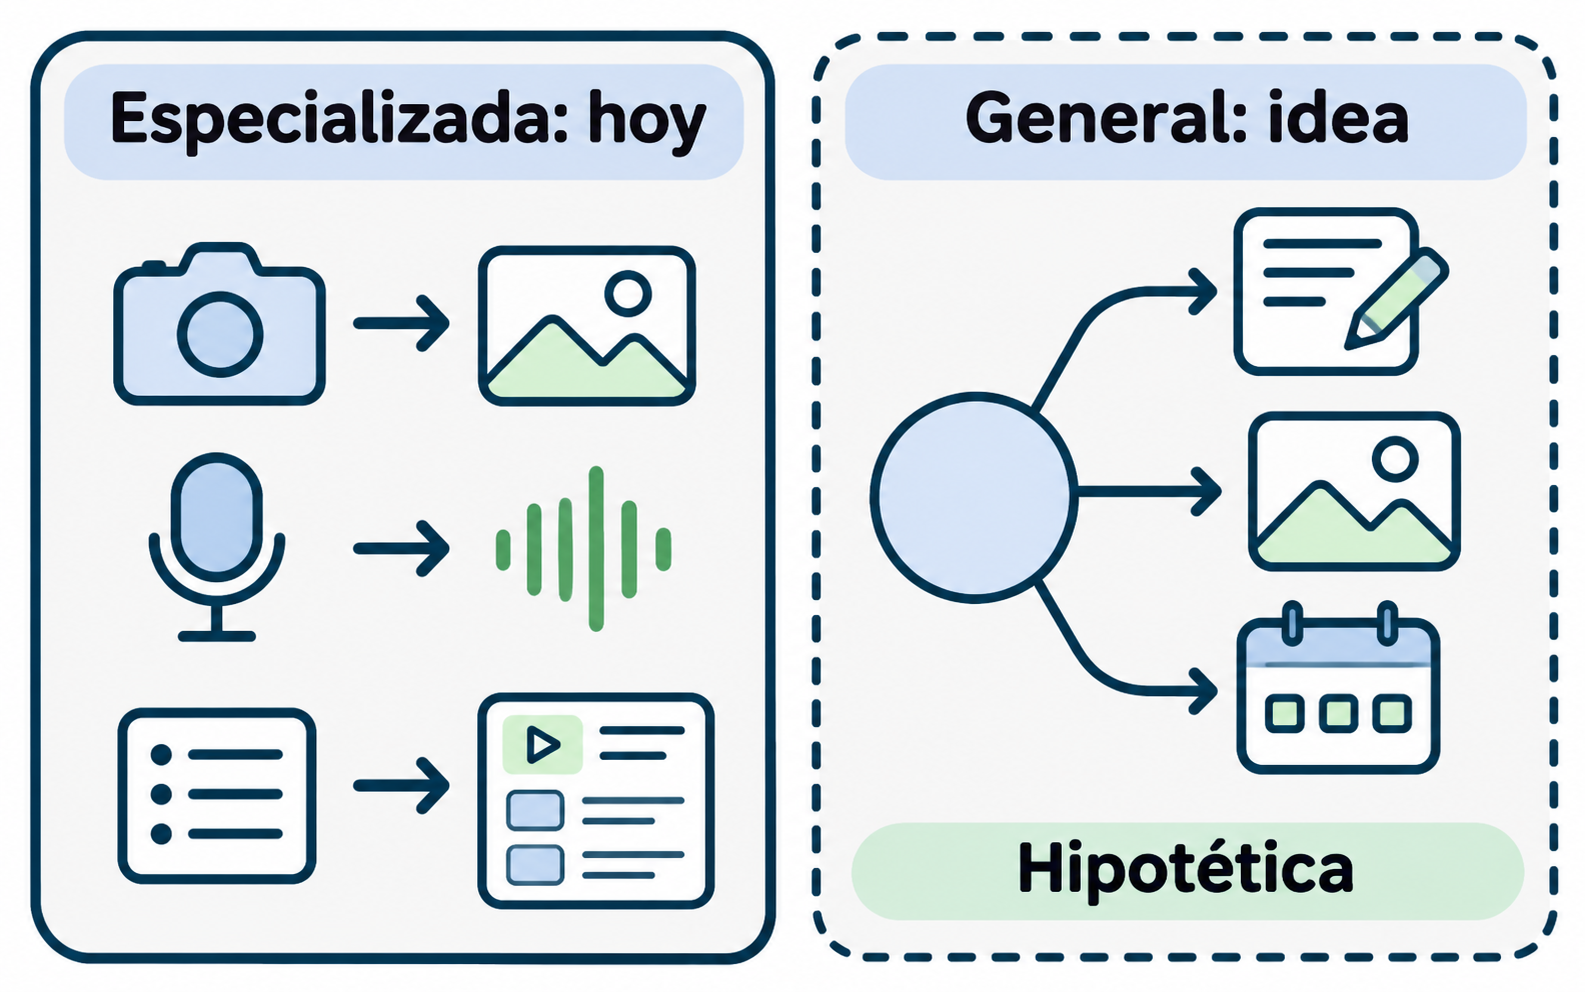
\includegraphics[width=\px{760}]{Especializada hoy vs. General hipotética.png}};
  \end{tikzpicture}
\end{frame}

% 19
\begin{frame}[plain]
  \begin{tikzpicture}[remember picture,overlay]
    \mentinode{54}{297}{1280}{19.5}{24}{Vamos a conversar con una IA}
    \mentinode{55}{435}{1280}{8}{14}{¿De qué formas podría ayudar la inteligencia artificial a estudiantes o familias de San Juan Bosco, en Morona Santiago? Da tres ejemplos sencillos.}
  \end{tikzpicture}
\end{frame}

% 20
\begin{frame}[plain]
  \begin{tikzpicture}[remember picture,overlay]
    \mentinode{54}{297}{1280}{19.5}{24}{Probemos con IA}
    \mentinode{55}{435}{1280}{8}{14}{Tres datos interesantes sobre San Juan Bosco.}
    \mentinode{55}{478}{1280}{8}{14}{Ideas para una familia agricultora.}
    \mentinode{55}{521}{1280}{8}{14}{Ideas para dar a conocer San Juan Bosco.}
  \end{tikzpicture}
\end{frame}

% 21
\begin{frame}[plain]
  \begin{tikzpicture}[remember picture,overlay]
    \mentinode{54}{297}{1280}{19.5}{24}{Sigamos explorando}
    \mentinode{55}{435}{1280}{8}{14}{¿Cómo podría la tecnología ayudar a cuidar plantas y animales?}
    \mentinode{55}{478}{1280}{8}{14}{¿Cuándo no conviene confiar completamente en una respuesta de IA?}
    \mentihint
  \end{tikzpicture}
\end{frame}

% 24
\begin{frame}[plain]
  \begin{tikzpicture}[remember picture,overlay]
    \mentinode{54}{297}{1280}{19.5}{24}{¿Qué aprendimos hoy?}
    \mentinode{55}{435}{1280}{8}{14}{\textbullet\ Escribe tres cosas que aprendiste hoy}
    \mentinode{55}{478}{1280}{8}{14}{\textbullet\ Escribe una pregunta que todavía tengas}
  \end{tikzpicture}
\end{frame}

\end{document}
